\chapter{Overview}
\label{chap:chapter-1}


Black holes and neutron stars are the most compact objects in the known universe.  
The mergers of these two objects,
 whether mixed in the form of black hole-neutron star systems or alike in the form of double black hole and double neutron star systems systems,
 are a primary source of gravitational waves.  
These objects form from massive stars,
 with masses $M\gtrsim 8\,M_{\odot}$,
 whose cores collapse from having burnt all their fusible material and thereby
 losing essential support from gas pressure.
Neutron stars result from supernova on the smaller-mass end of this population,
 and are self-supported against gravitational collapse by degenerate neutron gas pressure,
 not by burning fuel,
 and with masses ranging between $\sym (1-2)\,M_{\odot}$.
Smaller mass stars $M < 8\, M_\odot$ collapse into white dwarfs,
 which are self-supported by degenerate electrons.  
Fermi pressure from an electron gas is not as strong as that of a neutron gas,
 so white dwarfs cannot be supported unless they have masses $M\lesssim 1.4\,M_{\odot}$,
 the Chandrasekhar limit.  
Lastly, for masses larger than $M\gtrsim 10\,M_{\odot}$,
 supporting pressure of any kind cannot sustain an equilibrium with gravity.  
These collapses result in stellar-mass black holes.

Neutron stars are incredibly interesting species of exotic matter. 
During their formation from core-collapse supernovae,
 they collapse to a density close to that of nuclei.
Objects of such extreme densities have areal radii of $\sym 10 \textrm{km}$,
 smaller than the distance between Pullman, WA and Moscow, ID.
While dangerous, 
 you could bike around an area containing the entire mass of our solar system (plus some) in a single day.
Neutron stars are very compact.
Quantitatively, the compactness of an object is a measure of the how much mass is within an enclosed surface.
Compactness is unitless and defined by $\mathcal{C}\equiv G M/c^2 R$.
The factor $G M/c^2$ in the compactness paramater is the \textit{Schwartzchild radius},
 which when comparable to a stellar radius means general relativity plays an important role.
For reference,
% the compactness of the earth and sun are
% $\mathcal{C}_\textrm{E} \sim 10^{-10}$
% and
% $\mathcal{C}_{\odot} \sim 10^{-6}$,
 the Sun, TRAPPIST-1 and a typical white dwarf are
 $\mathcal{C}_{\odot} \approx 4 \times 10^{-6}$,
 $\mathcal{C}_\textrm{T-1} \approx 0.7\,\mathcal{C}_{\odot}$
 and
 $\mathcal{C}_\textrm{WD} \approx 1.8 \times 10^{-4}$,
 respectively.
Clearly general relativity does not play a major role in these stars.
Meanwhile, for neutron stars and black holes, the compactnesses are 
 $\mathcal{C}_\textrm{NS} \approx 0.15$
 and
 $\mathcal{C}_\textrm{BH} = 0.50$.
At this end of the compaction scale, general relativity cannot be ignored.  The spacetime surrounding these two objects has extreme curvature.

To further get a sense for how dense neutron stars are, a quick back of the envelope calculation is to consider a $M_\textrm{NS} = 1.4 M _\odot$ star, which when divided by the mass of a neutron accounts for $\sym 1.7 \times 10^{57}$ total nucleons.
If the nucleons are homogeneously dispersed in this star, with areal radius of $12\,\textrm{km}$, the separation between them is then $\sym 1\,\textrm{fm}$.
From scattering experiments, we know the spacing of nucleons to be $\sym 0.8\,\textrm{fm}$ so the baryons are essentially touching.
In this compactness regime, we expect all fundamental forces to be important.
Nuclear forces strongly contribute to the pressures in the inner and outer core.
The crust is mostly supported by coulomb forces which in equilibrium yield lattice structures.
An isolated neutron star is in $\beta$-equilibrium, which is governed by the weak force and completely breaks down when the star is disrupted in extreme spacetime.

%
%\textbf{TODO: Add more physics?}
%Due to the conservation of angular momentum, neutron stars---much smaller in breadth than their mothers---have very high spins.
%
%Magnetized neutron stars with extreme spins, or pulsars that emit X-rays,
% have received immense interest within the community.
%
%
%\section{Binary scenarios}
%
%Shibata et al determined that black hole-neutron star binaries that produce gravitational waves fall into three categories: (1) if the neutron star falls directly into the black hole, the waveform is similar to that of a double black hole waveform; (2) if the neutron star disrupts far from the innermost stable circular orbit (ISCO), no merger or ringdown signal is observed; (3) if the neutron star disrupts close to the ISCO, inspiral and merger waveforms are observed but with a reduced ringdown signal.
%We expect tidal deformation to occur when the tidal force from object A overcomes the self-gravity of object B.  In the case of our black hole-neutron star systems, the separation distance in which tidal deformation occurs is given by
%\begin{align}
%d_{\rm TD} \sim R_{\rm NS} q^{1/3}
%\end{align}
%where q is the dimensionless mass ratio $q \equiv M_{\rm BH} / M_{\rm NS}$.
%
%\textbf{TODO: Finish...}

\section{Coalescence \& merger and their observables}
\label{sec:observables}

\paragraph{Inspiral and Gravitational waves}
A number of observable phenomena involving black hole-neutron star and double neutron star mergers are considered.  
The orbits of compact binaries decay as gravitational waves carry energy away from the system, causing them to inspiral and eventually merge.  
Gravitational waves were observed by the advanced Laser Interferometer Gravitational-Wave Observatory (aLIGO) network ~\cite{aLIGO2} on September 14, 2015 ~\cite{LIGOVirgo2016a,Abbott:2016nmj}. 
The SXS collaboration simulated thousands of double black hole inspirals and mergers with numerical relativity to probe the seven dimensional parameters space (mass ratio, two spin alignments for each object, and their spin magnitudes).  
From the SXS catalog, the observation of the GW150914 event was determined to have black holes with masses $29 M_\odot$ and $36 M_\odot$, forming a resulting $62 M_\odot$ black hole, radiating $~3 M_\odot c^2$ of energy away from the system.
While the detection of mixed binary mergers is likely to only account for 1-2\% of measurable events from aLIGO, additional information on the electromagnetic spectrum is observable during and after merger~\cite{1976ApJ...210..549L,Li:1998bw,Roberts2011,Kasen:2013xka,Tanaka:2013ana}. 

\paragraph{Merger and Kilonovae}
~\cite{Shibata:2009cn} determined that black hole-neutron star binaries that produce gravitational waves fall into three categories: 
(1) if the neutron star falls directly into the black hole, the waveform is similar to that of a double black hole waveform; 
(2) if the neutron star disrupts far from the innermost stable circular orbit (ISCO), no merger or ringdown signal is observed; 
(3) if the neutron star disrupts close to the ISCO, inspiral and merger waveforms are observed but with a reduced ringdown signal.
In our study, we have focused on the latter. 
A highly spinning, stellar-massive black hole will cause maximal disruption, causing a large portion of the stellar matter to become unbound and get ejected from the system.
In the ejecta, the fluid expands and cools, where r-process nucleosynthesis takes place.  
Neutrons are absorbed by heavy nucleii, radiating optically bright neutrinos thorough the interstellar medium. 
After a timescale of days, the unstable elements decay, which heats the ejecta, causing bright afterglows (kilonova) that can be observed with ground- and space-based optical and infrared detectors ~\cite{tanvir2013kilonova}.

\paragraph{Post-merger and sGRB's}
A large amount of bound material will remain in the post-merger system.  
The fluid circularizes around the black hole, causing shock heating prior to axisymmetrization. 
A large portion of bound material in the tail crashes back into the disk, causing further heating.
Magnetic effects from the Blandorf-Znajek effect or by neutrino-antineutrino annihilation energy deposition near the poles of the post-merger accretion disk can drive ultra-relativistic jets at the black hole poles, which may be observable on the order of seconds, or as long as the disk is still accreting.
The jet could beam high-energy gamma ray photons---an observable short-duration gamma ray burst (sGRB).
Neutrino-driven winds could also contribute to strong disk outflows, contributing to post-merger kilonovae.

What's important here is that having a near-infrared or sGRB counterpart to the gravitational wave signal provides information that can be detected on multiple astronomical instruments, so dubbed multi-messenger astronomy.
Second, transients that emit near the infrared spectrum occur at different timescales to gravitational waves after the merger event.
Kilonovae formed in the outflowing tail material should be detectable seconds after the accompanying gravitational wave.  



\section{Brief overview of the inspiral, merger, and post-remnant dynamics}

The neutron star and the black hole coalesce and inspiral due to radiation of gravitational waves in the first $(10-20)$ms of the simulations considered in this work.  
The actual inspirals may last much longer than this for events in our universe, but we only evolve the late inspiral for computational cost reasons, and less computationally expensive models (post-Newtonian) can accurately evolve early times.
The dynamics of the merger and post-merger processes are of key interest to our study.
The merger phase begins with the neutron star rapidly distorting due to tidal deformation of the black hole.
In a typical merger, three processes can happen depending on the binary mass and spin configurations~\cite{Shibata:2009cn}.  The neutron star will plunge directly into the black hole without disrupting, and the gravitational signal will be similar to double black hole waves; the star will disrupt well outside the innermost stable circular orbit (ISCO), leaving no merger or ringdown impression on the waveform; or, in the intermediate region where the star disrupts close to the ISCO, the star will maximally disrupt, inspiral and merger are imprinted on the wave signature while the ringdown phase does not.

Our models use mass and black hole-spin configurations that allow for the intermediate scenario.  
First, the star begins to distort as it gets close to the black hole, where tidal forces become large, with a timescale on the order of $(2-4)$ms.  
The star further deforms into a stream as it begins to plunge toward the black hole.  
Gravitational torques cause some of the fluid to become unbound, most matter accretes, and the accretion rate accelerates to a maximum at the onset of merger.  
At that stage, the neutron star fluid is stretched thin near the horizon, with a large, kicked tail expanding outward.
After the accretion rate begins to decelerate and eventually reach a local minimum, the ingoing stream of matter with sufficient angular momentum intersects with the bound portion of the tail, which shocks the remnant fluid, causing heating, allowing stability of the early-formation disk via angular momentum transfer through accretion.
This rapid onset of merger happens quickly, lasting $\sym 1$ms.
The early formation disk, hereafter \textit{protodisk}, undergoes admixture with the tidal tail, in an asymmetric mass transfer of fallback onto the protodisk and accretion onto the black hole.
The rest of the unbound material escapes the system, homologously expanding into the interstellar medium.
On much longer timescales but within thermal timescales ($\sym 40$ms), as fallback depletes, the remnant system begins to axisymmetrize and secularize from the outgoing tail.
We provide an overview of these epochs around the merger time in Figure \ref{fig:timesnaps}.

\begin{figure}
	\centering
	\begin{subfigure}[b]{0.475\textwidth}
		\centering
		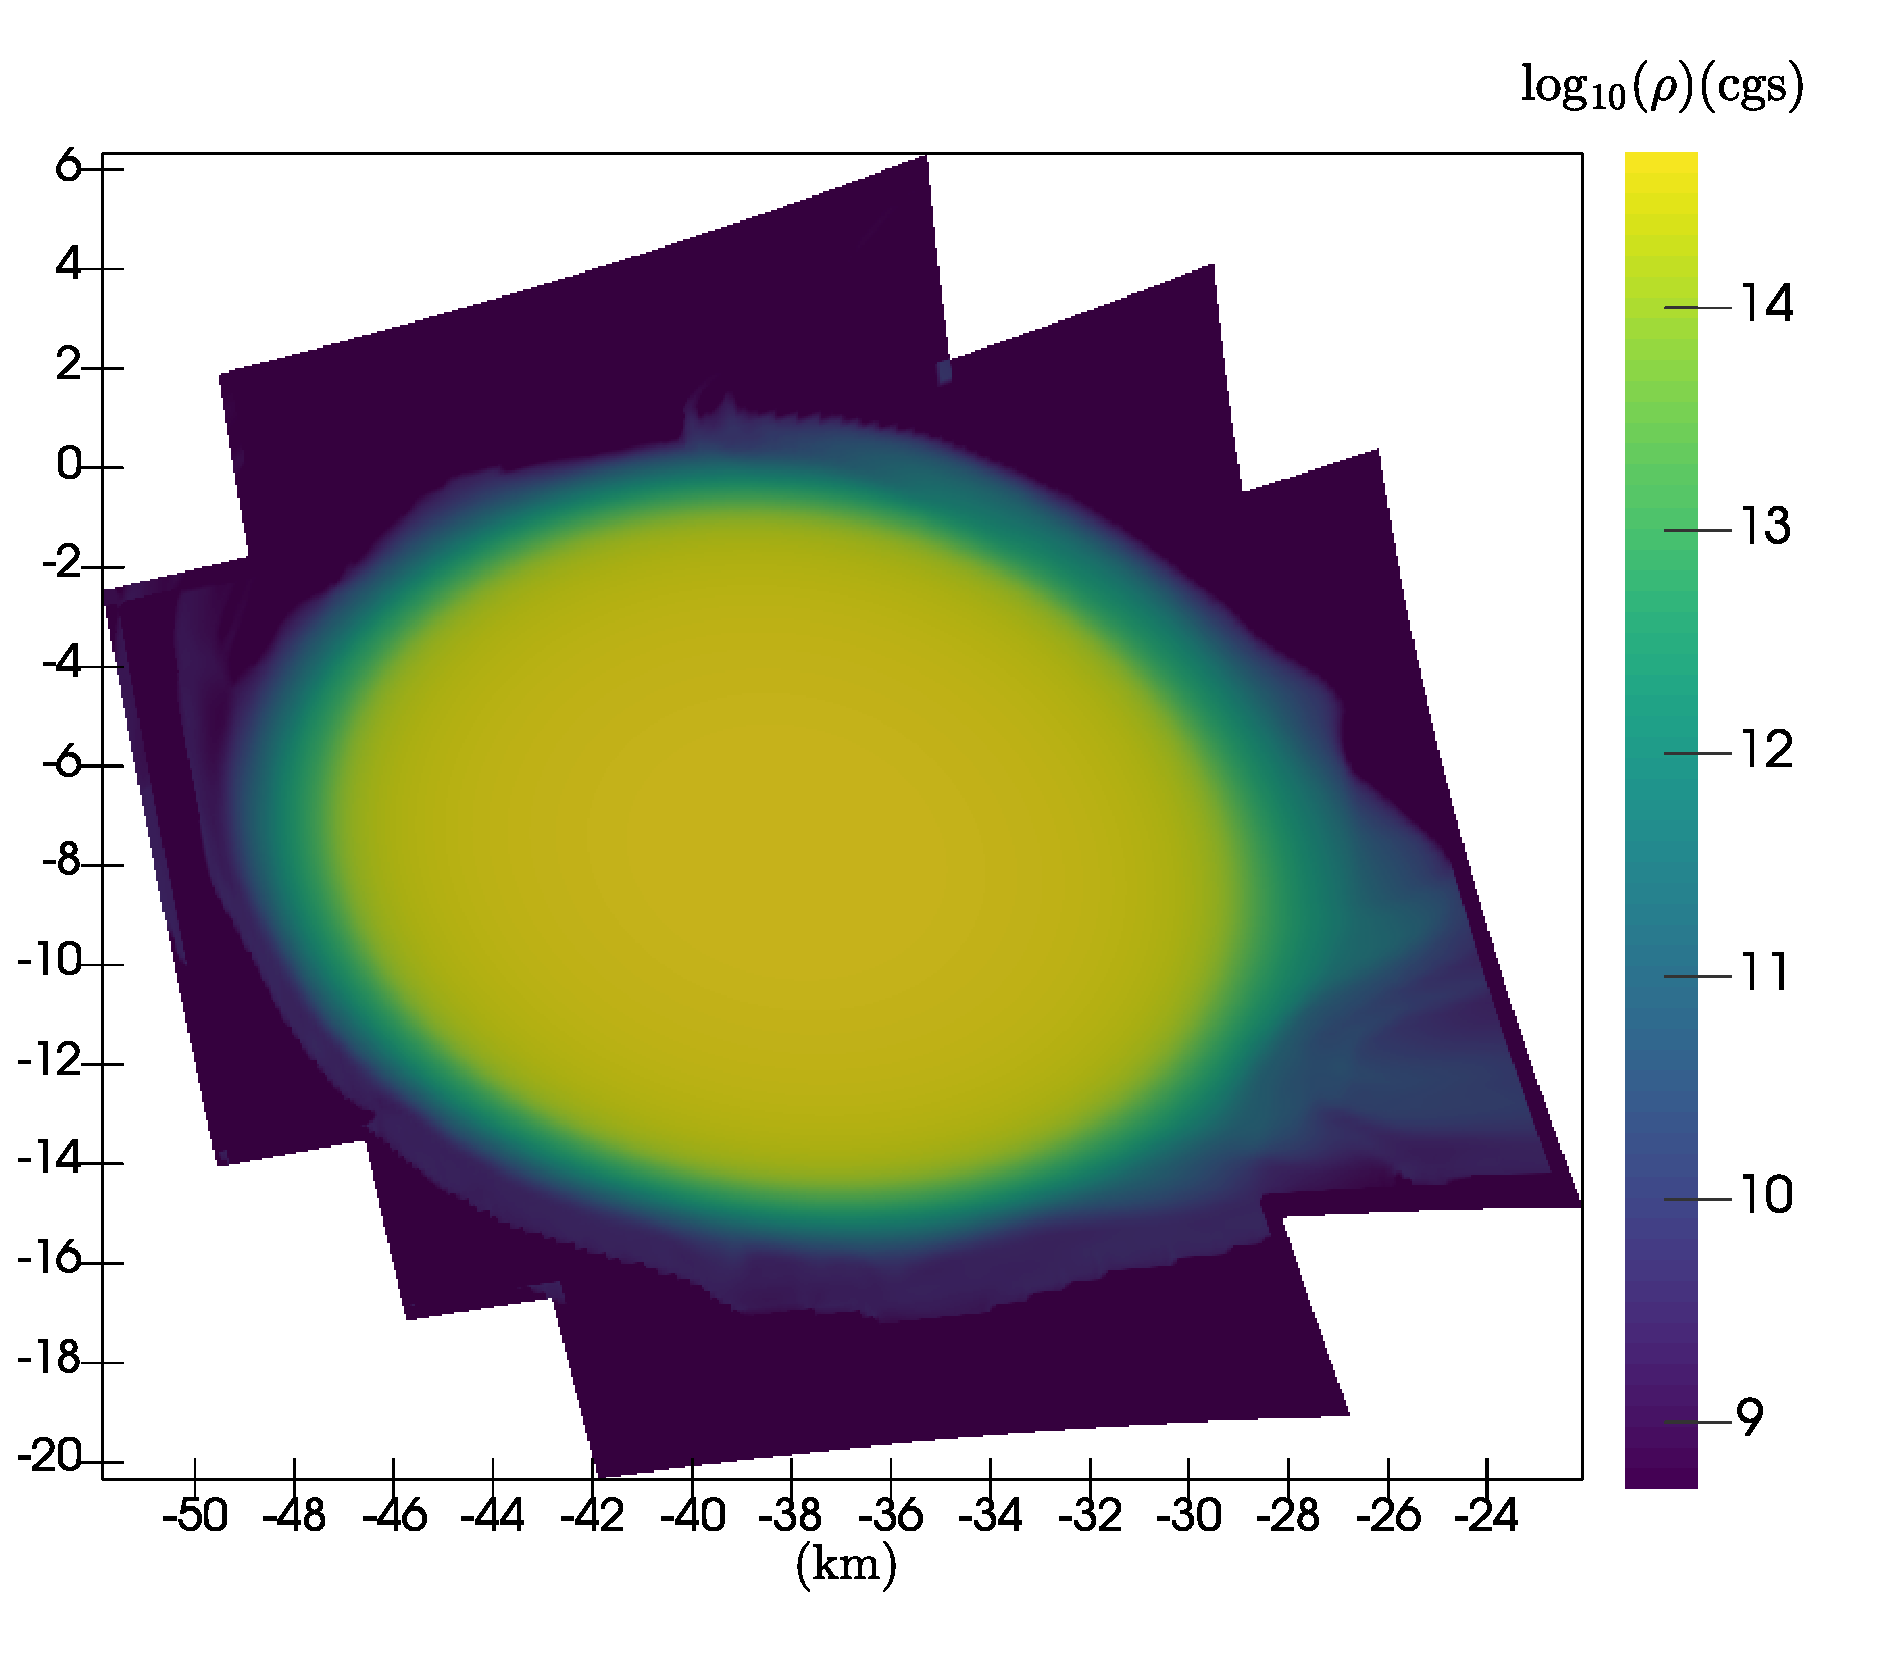
\includegraphics[width=1.0\linewidth]{images/rho_DD2_M12-m4ms-inertial}
		\label{fig:rho_M12_DD2_m4ms}
	\end{subfigure}
	\begin{subfigure}[b]{0.475\textwidth}
		\centering
		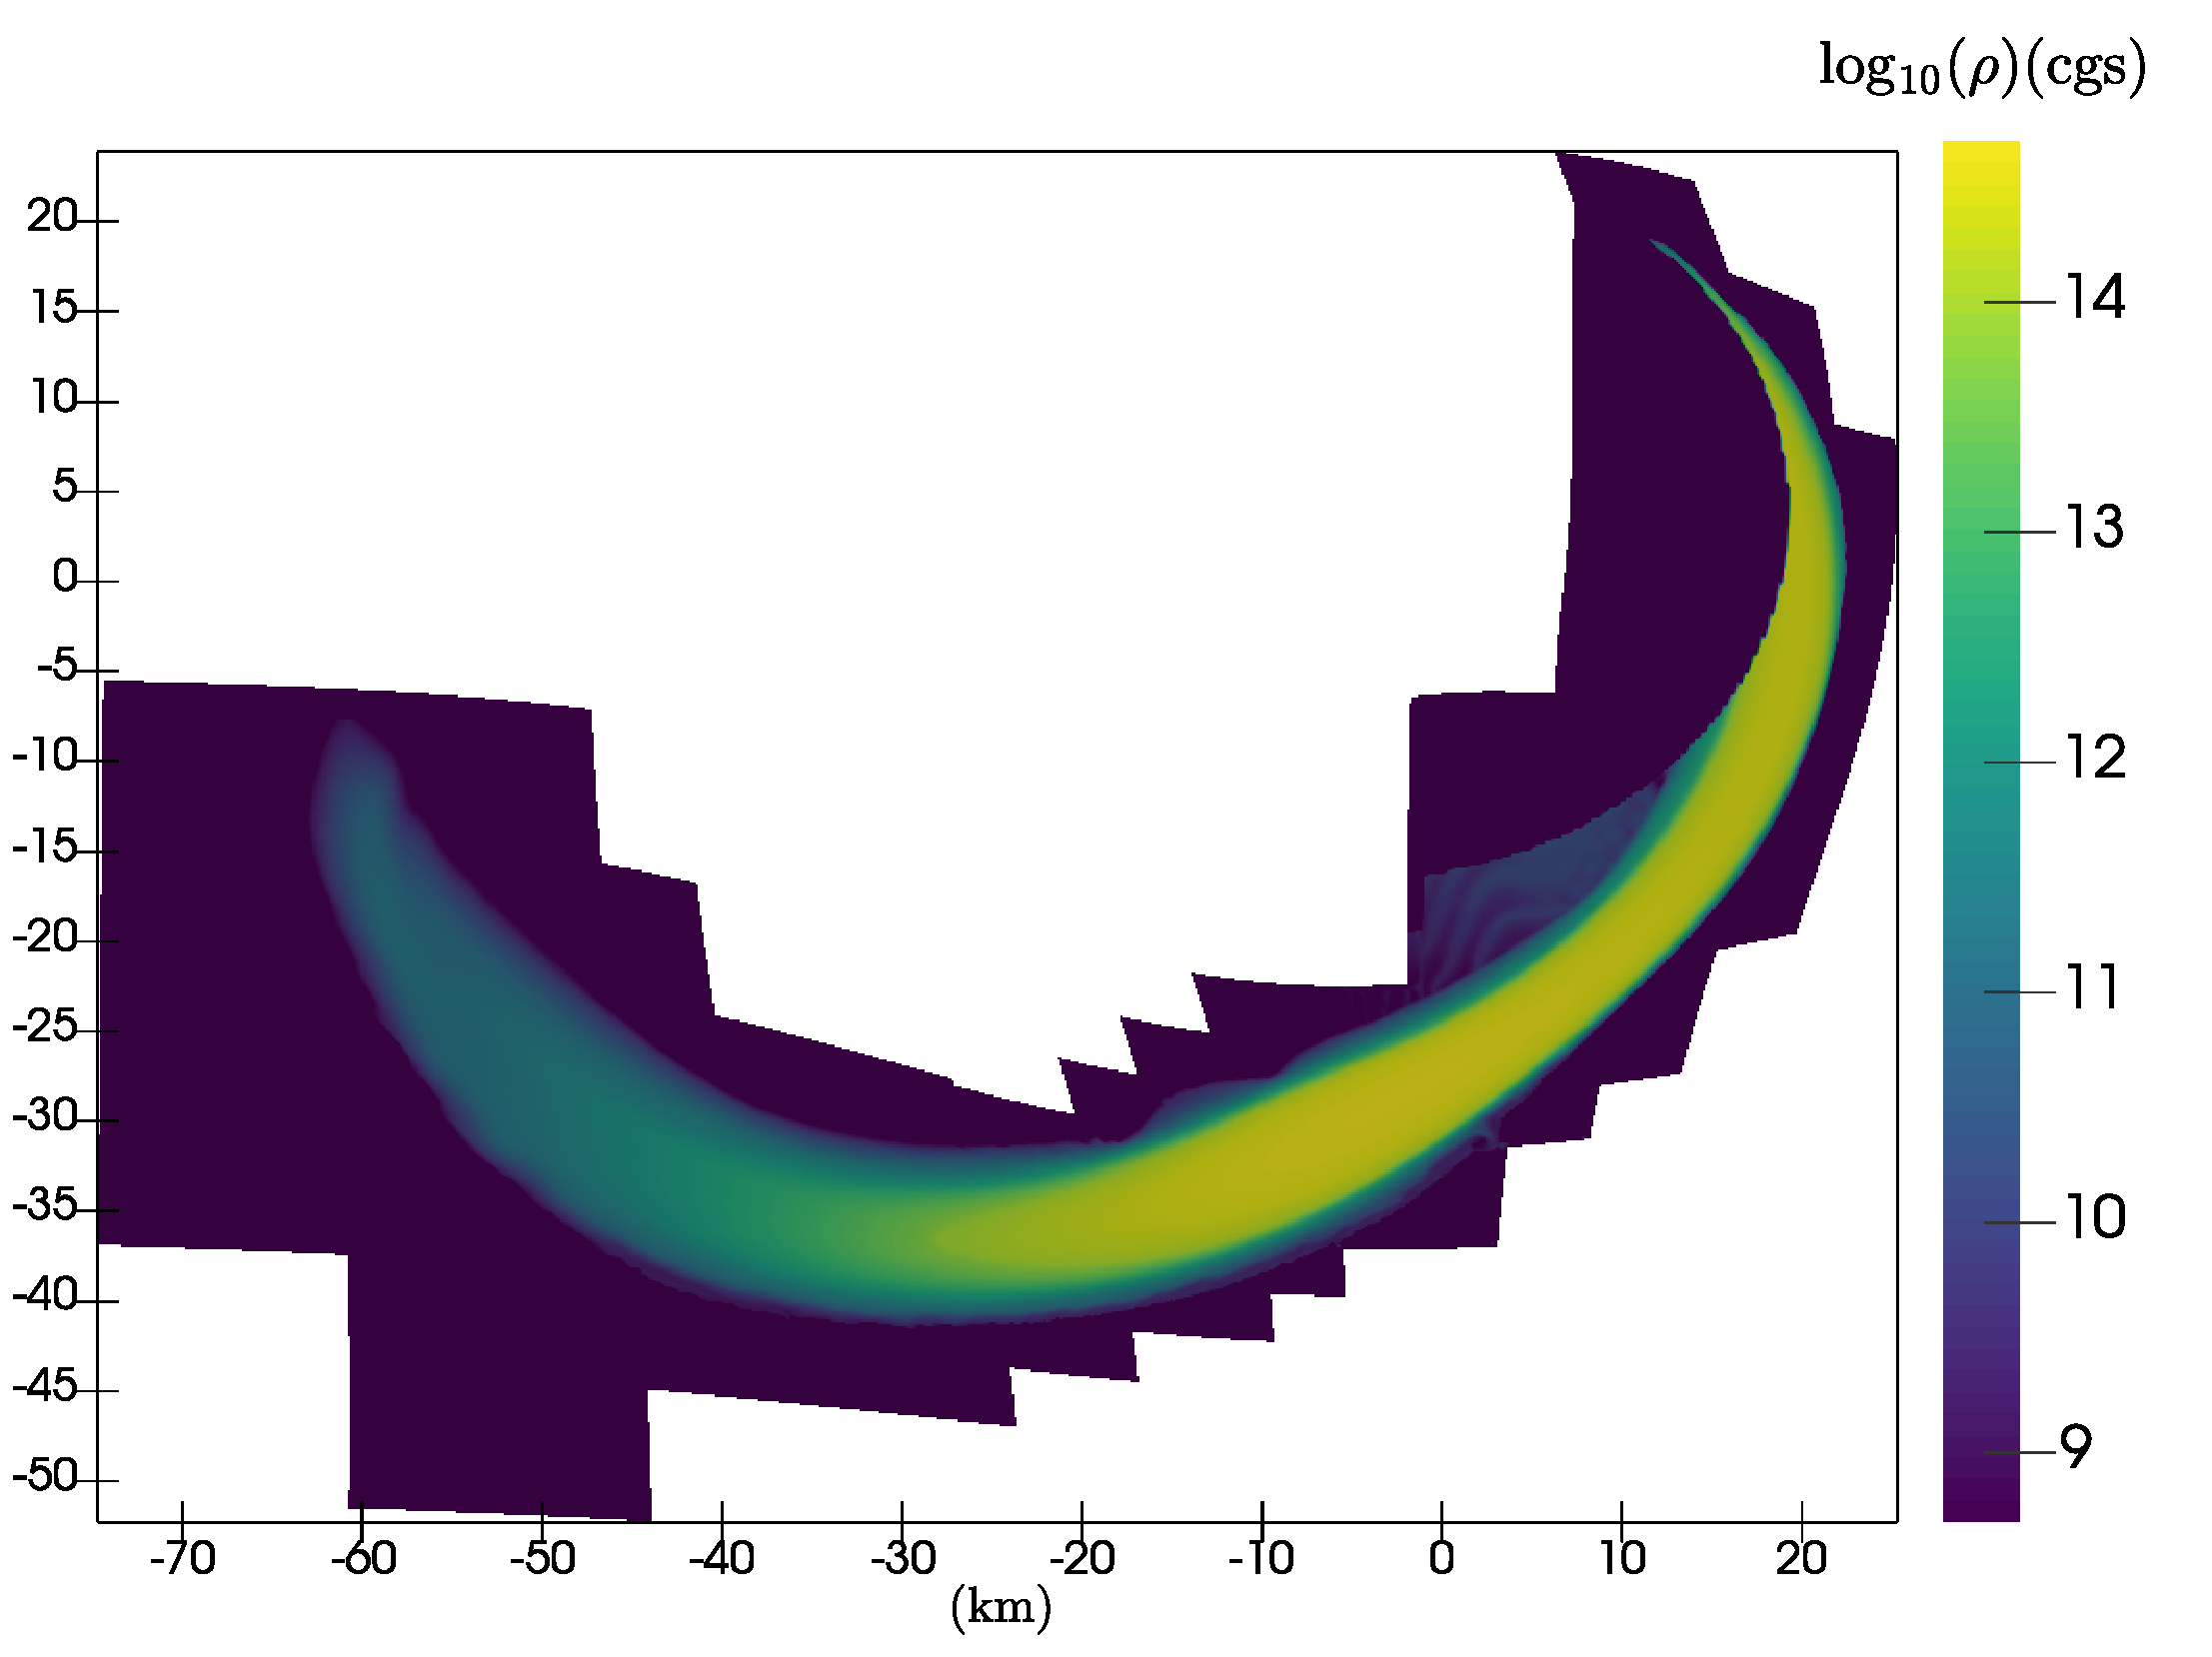
\includegraphics[width=\linewidth]{images/rho_DD2_M12-m1ms-inertial}
		\label{fig:rho_M12_DD2_m1ms}
		\centering
	\end{subfigure}
	\begin{subfigure}[b]{0.475\textwidth}
		\centering
		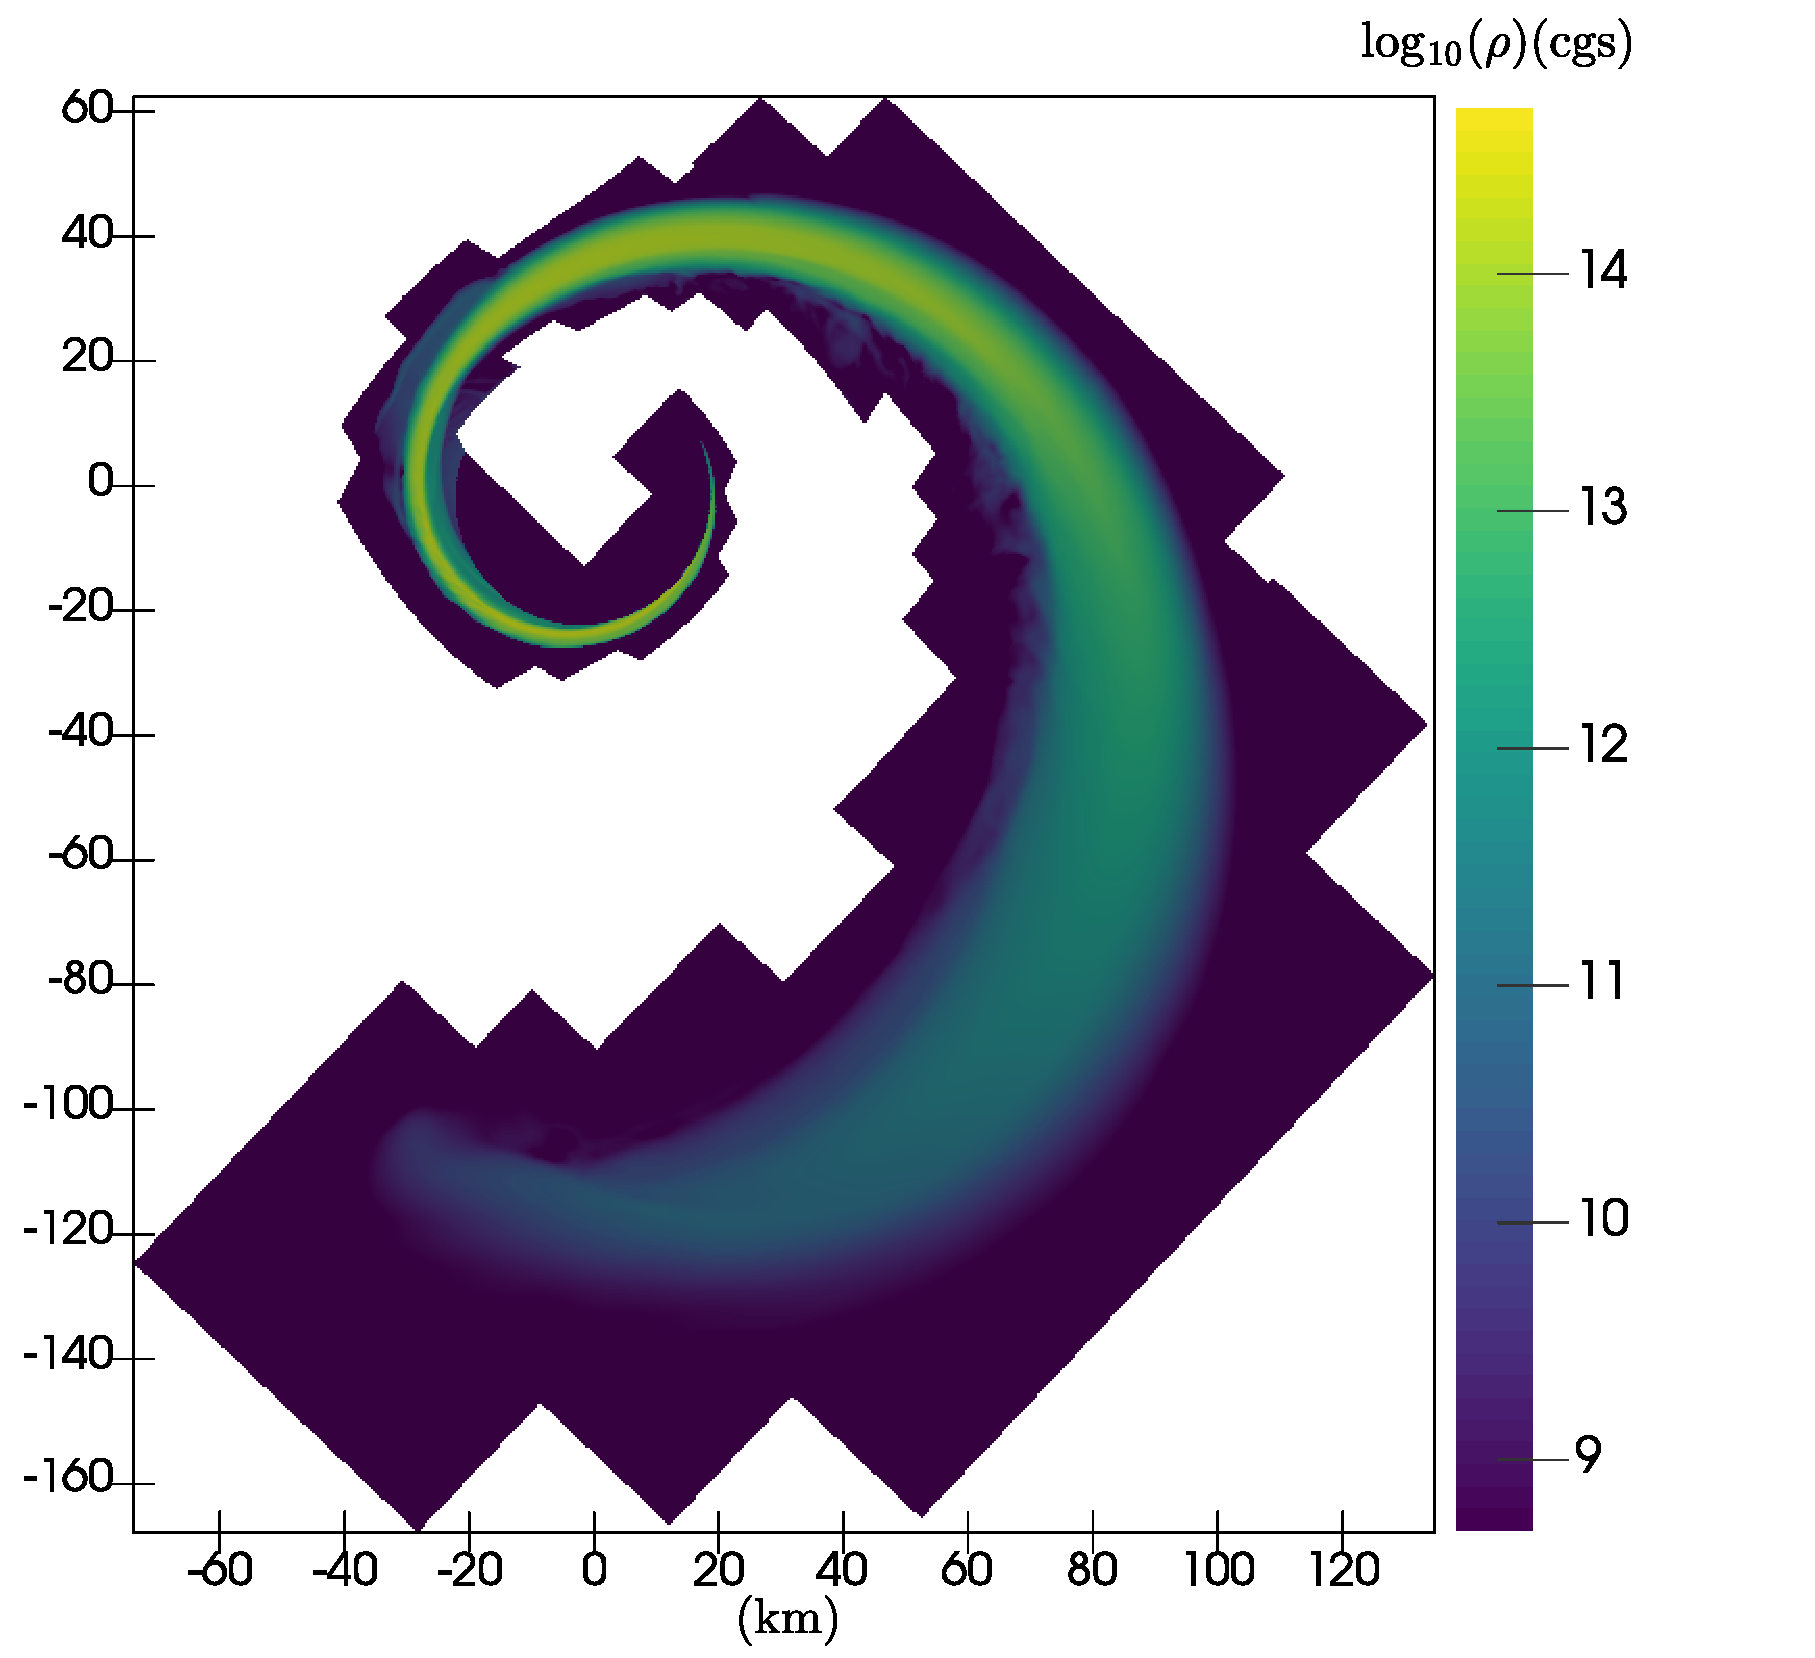
\includegraphics[width=\linewidth]{images/rho_DD2_M12-merger-inertial}
		\label{fig:rho_M12_DD2_0ms}
	\end{subfigure}
	\begin{subfigure}[b]{0.475\textwidth}
		\centering
		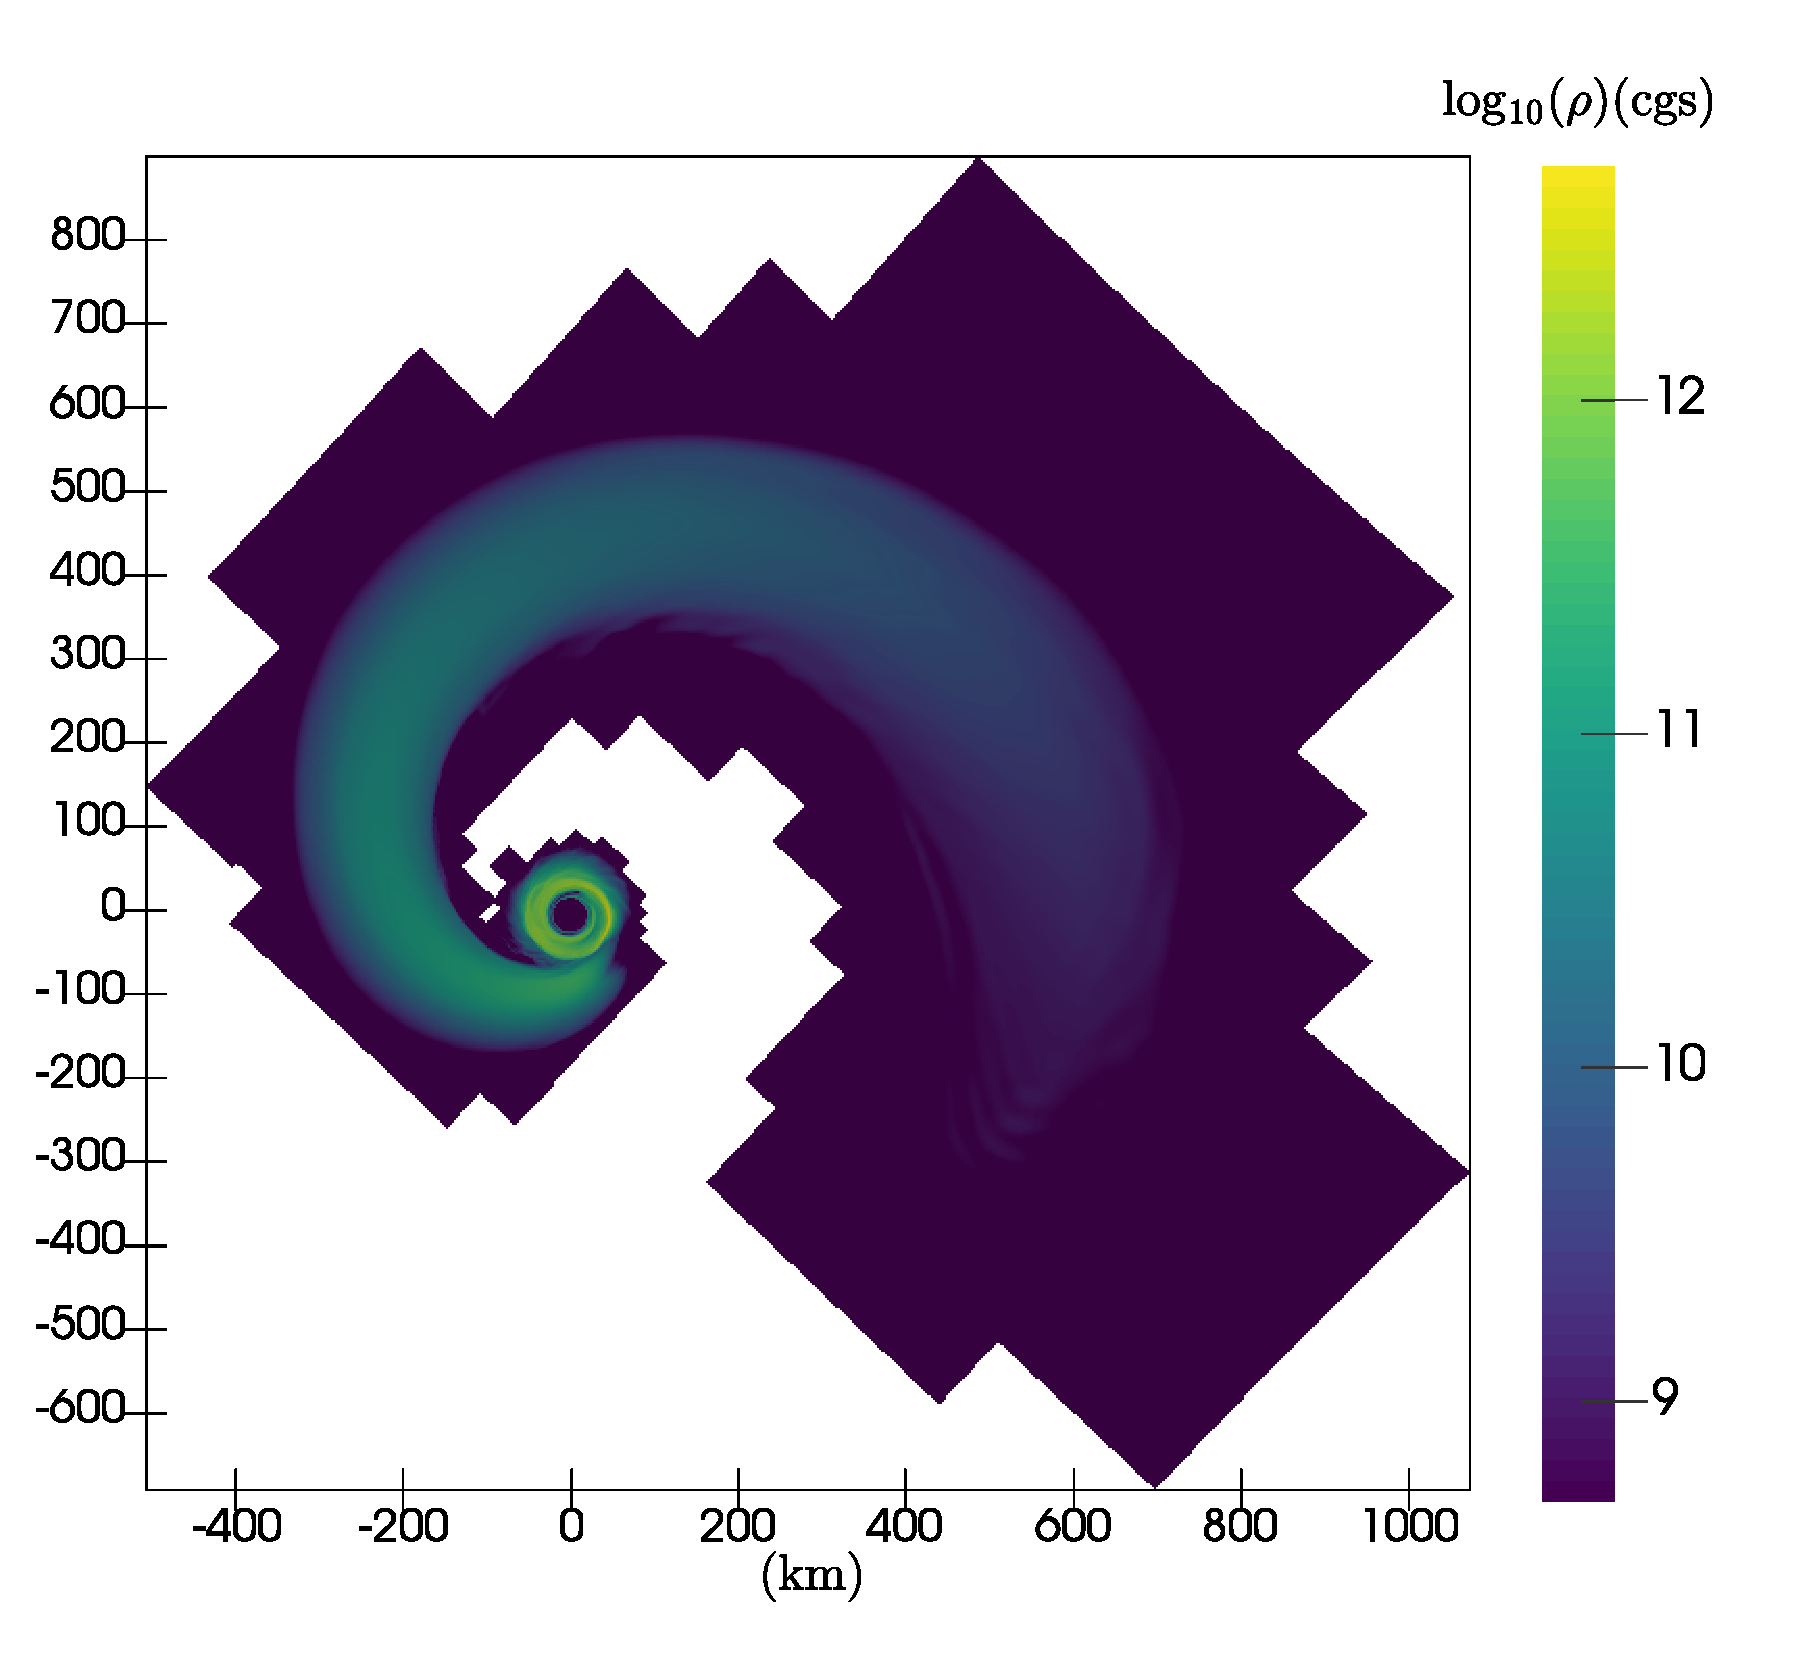
\includegraphics[width=\linewidth]{images/rho_DD2_M12-5ms-inertial}
		\label{fig:rho_M12_DD2_5ms_}
	\end{subfigure}
	\caption[Time lapse of fluid evolution before and after merger]{
		Baryon density profiles on the equatorial plane where the initial neutron star has a mass of $M_{\rm NS} = 1.2 M_{\odot}$.  Each picture corresponds to what we refer to as merger time: when $50\%$ of the neutron star material has been accreted onto the black hole.
		\textit{Top left:} 4ms before merger, where star just begins to tidally deform.
		\textit{Top right:} 1ms before merger, where the star has now begun to plunge into the black hole.
		\textit{Bottom left:} Merger, at which point the fluid stretches into a very thin tidal stream that eventually crashes into the other end of the arm.
		\textit{Bottom right:} 5ms after merger.  The fluid has formed a protodisk around the black hole, being heated from its own asymmetries and interaction with the fallback matter. Low density regions in the outer tail are ejected from the system.
		We display all four epochs in the coordinates of the laboratory frame, noting that the grid continues to expand with the outflow from $\sym 2 R_{NS}$ in the top left panel to $\sym 10 R_{NS}$ during merger and then to the order of $\sym 100 R_{NS}$ $5$ms after.

	}
	\label{fig:timesnaps}
\end{figure}


\section{Presentation of this thesis}

%For as many enriching astrophysical scenarios involving neutron stars, there are an order of magnitude more people studying, simulating, and observing their progenitors, mergers, and companionship with other compact objects.
%This thesis could never begin without the work of all those that contributed to our knowledge of neutron star matter thus far, and a wishful attempt has been made to excise the less relevant but no less important subfields from our discussion.
First, it must be acknowledged that we are only studying one type of system involving neutron stars in this paper.  Neutron star-neutron star mergers also play a key role in the effort to model gravitational waves and their electromagnetic counterparts. 
Black hole-neutron star sources and the observable information we can extract from them will help us probe the nature of neutron star structure and predict the electromagnetic signals, specifically the properties of  their origins.

Alas, there is a decidedly chicken-and-egg problem to the order in which one begins to model stellar structure and how the star evolves in a dynamical system.
In a short manuscript, the theoretical overview for both can be done in some sense in just a few pages. 
However, the evolution system of the Spectral Einstein Code (\SpEC) is complex, requiring many nuances to not only explain how the fluid and Einstein equations are solved, but the modifications and controls that must be made to the grids they are evolved on.
And because the subject matter of this thesis is to study several nuclear-theory based, finite-temperature equations of state of neutron stars being violently disrupted by black holes, I have likewise chosen to have a separate chapter devoted to that salient detail of the star.
% still mulling over the order in which the EOS vs evolution equations are discussed

I have thus decided to structure this manuscript putting the emphasis first on the equation of state of neutron star matter in Chapter \ref{chap:chapter-2}, and then discuss the evolution of the relativistic fluid and Einstein's equations in Chapter \ref{chap:chapter-3}.  
I've done this for several reasons: 
in our simulations, the neutron star is constructed before evolution of the fluid variables, and only requires a solution of the equations of hydrostatic equilibrium (i.e. the Tolman-Oppenheimer-Volkoff equations) to model the star in isolation.  
After the star is constructed in isolation with the equation of state (in our simulations, only using a low temperature, one dimensional slice of the three-dimensional table), we place it in quasi-circular orbit around the black hole by solving the constraint equations for the metric field and determining the stellar profile and orbital frequency for quasi-equilibrum circular orbit.
These two objects inspiral in a decaying orbit, shedding away angular momentum in the form of gravitational waves.  
For our specific configuration, our stars do not plunge directly into the black hole, but disrupt into a stream of neutron-rich matter, and coalesce into a neutrino-bright ``protodisk'' infusing cooler material from the infalling portion of the tidal tail. 
Most of the matter accretes onto the black hole, but the remaining chunk either gets flung from the system if the matter is unbound, or circularizes into an accretion disk with the remaining bound matter falling back.
